\begin{document}
  \chapter{Conclusion}
    \section{Conclusion on Database Implementation}
      \paragraph{}
        This project makes us realized that ER Database is very useful and very worthful to study because it allows us to
        design the database using the ER diagram which is very semantic concept. Also learning SQL allows us to send queries to
        view and edit those tables in the database.
      \paragraph{}
        There are a few points, besides query commands, we believed very important to our project.
      \begin{itemize}
        \item Views - Allows us to create a virtual table that could be used for securely views the table, also it facilitate viewing complex join of tables
        \item Routines - Very important function of SQL because they help us a lot in calling a series of SQL commands without explicitly call all of them
        \item Foreign Key - Allows data to be verify whether it is correct and relate to the parent table or not.
      \end{itemize}
      \begin{center}
        \begin{figure}[!h]
          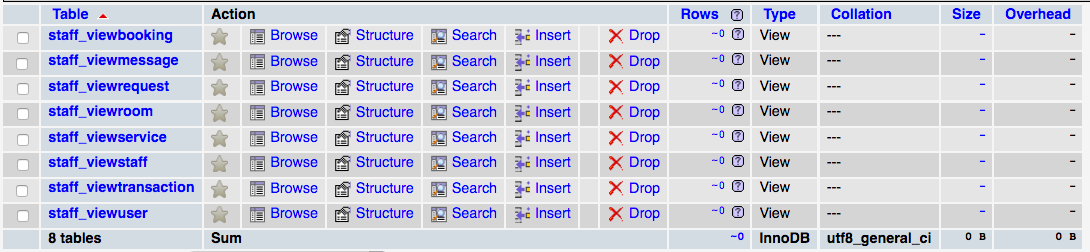
\includegraphics[width=\textwidth]{views}
          \caption{Some views we used in the project}
        \end{figure}

        \begin{figure}[!h]
          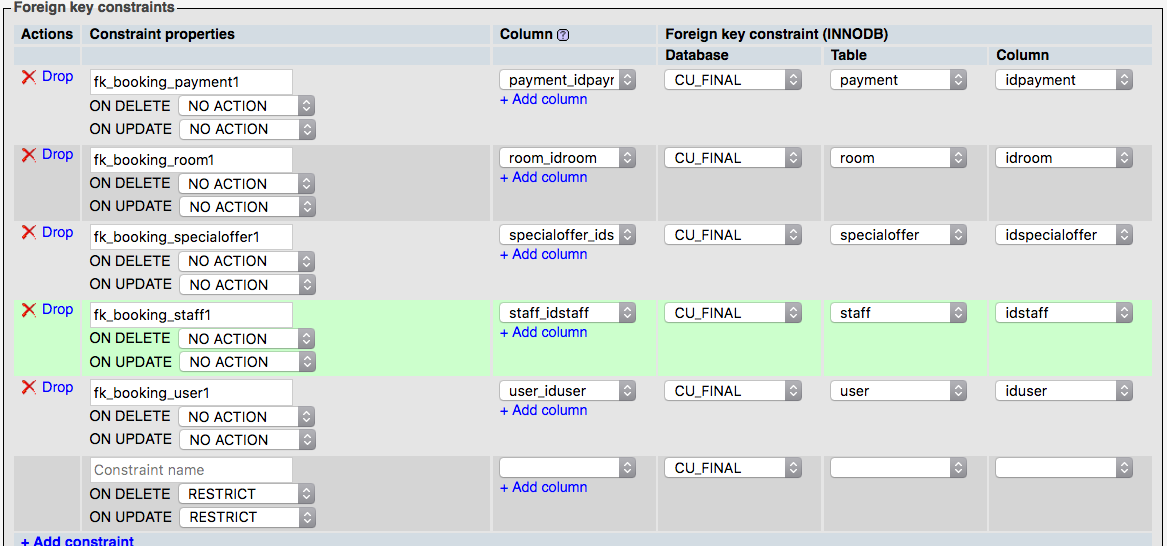
\includegraphics[width=\textwidth]{foreignkey}
          \caption{Foreign Key constrains}
        \end{figure}
      \end{center}
      \paragraph{}
        Those points are very important and helped us a lot.

    \section{Conclusion on Web Implementation}
      \paragraph{}
        We gained a lot of software development experience from working together as it taught us to write thousand lines of code with several weeks working period.
        We learned to use many tools to develop this project including developing tools such as
      \begin{itemize}
        \item PHPMyAdmin - use for viewing tables in GUI mode.
        \item MySQL CLI - use for querying and doing works in CLI mode.
        \item MySQL Workbench - use for designing the DB from ER Diagram.
        \item Text Editors - Our team use Atom for developing the project
        \item GitHub - use for version control system
      \end{itemize}
      \begin{center}
        \begin{figure}[!h]
          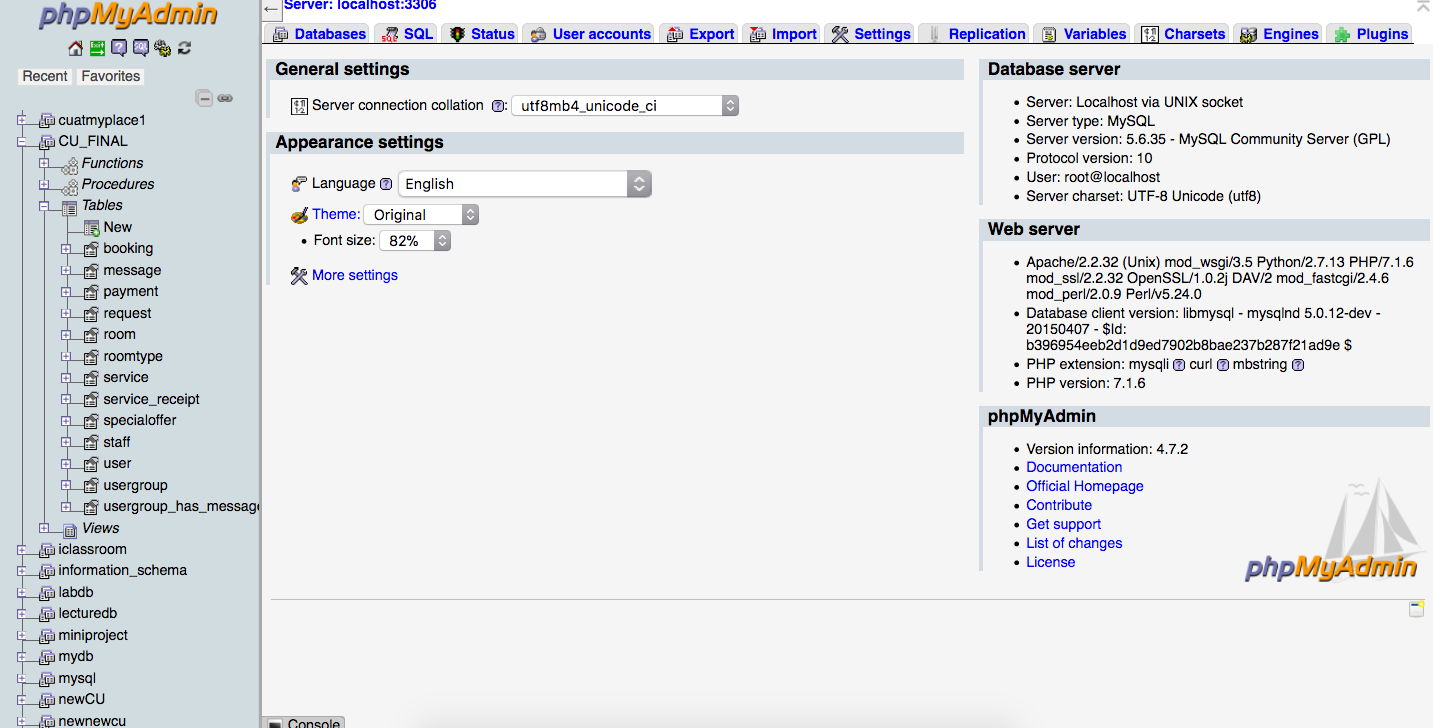
\includegraphics[width=\textwidth]{phpmyadmin}
          \caption{PHPMyAdmin}
        \end{figure}
        \begin{figure}[!h]
          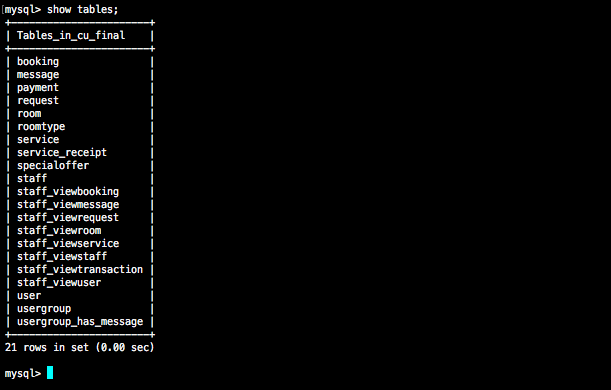
\includegraphics[width=\textwidth]{terminal}
          \caption{Running MySQL in Terminal}
        \end{figure}
        \begin{figure}[!h]
          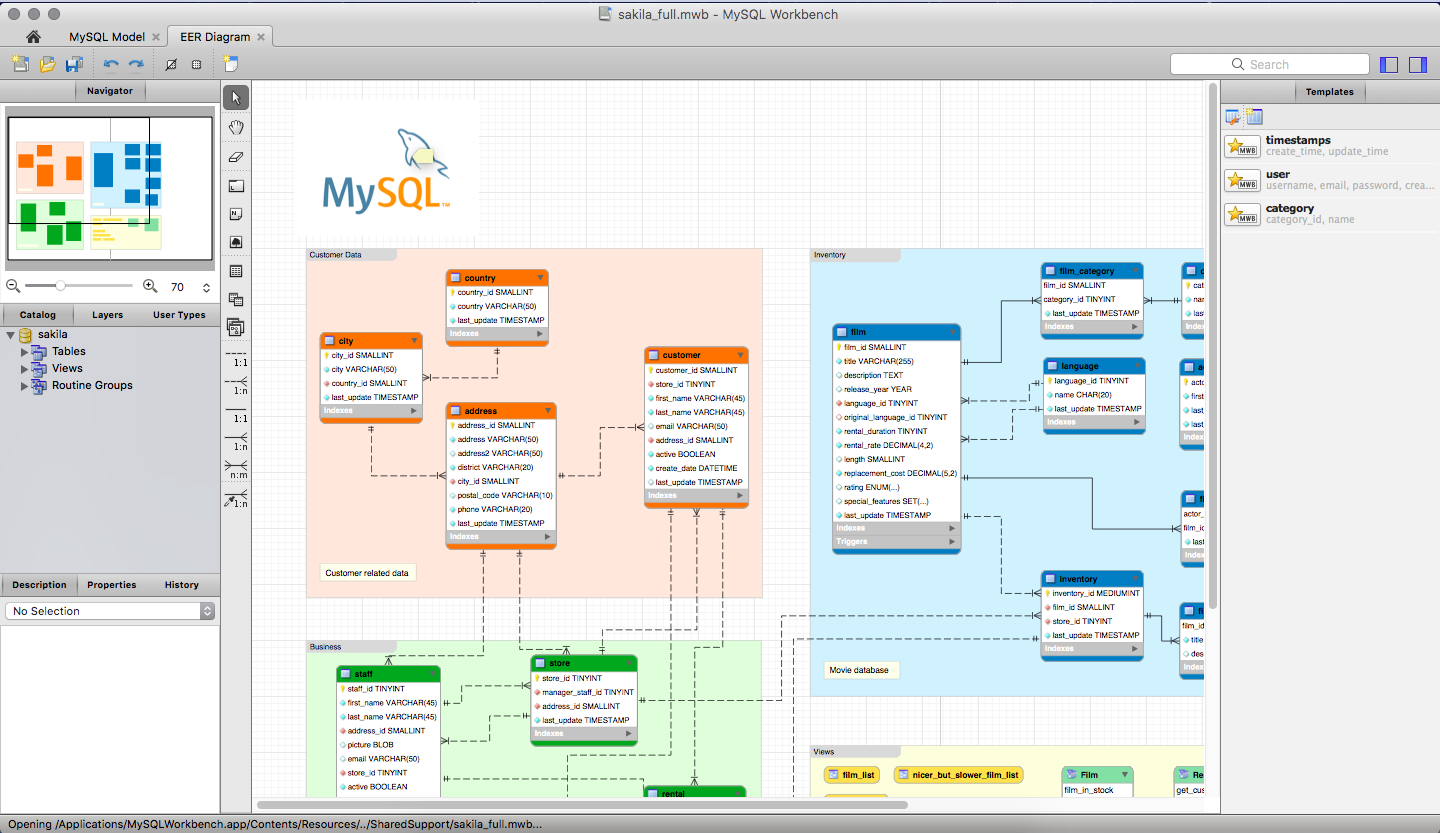
\includegraphics[width=\textwidth]{workbench}
          \caption{MySQL Workbench}
        \end{figure}

        \begin{center}
          \begin{figure}[!h]
            
\includegraphics{atom}
            \caption{The Editor we were using}
          \end{figure}
        \end{center}

        \begin{figure}[!h]
          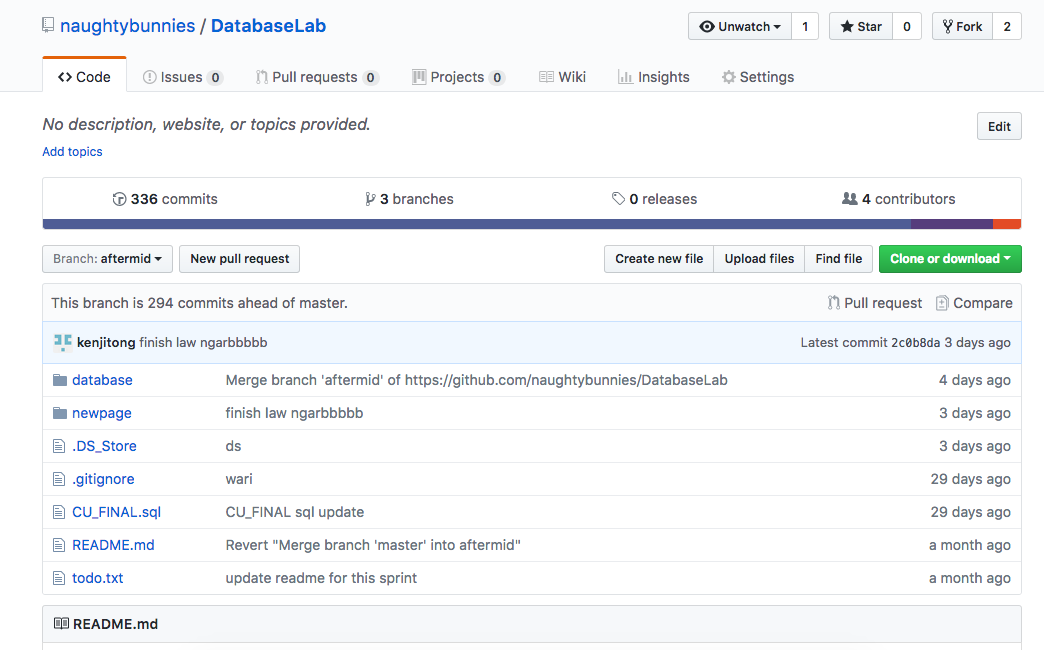
\includegraphics[width=\textwidth]{git}
          \caption{Github : This is the actual repository of the project}
        \end{figure}
      \end{center}

      \paragraph{}
        Because of those points mentioned above, We did learned a lot from doing the project. But the project itself still has a lot of room for
         improvemnt. It still could be developed using CSS Framework for prettier UI or use JavaScript for dynamic webpage for better experience.
         The system itself still need to be tested in practical use in order to gain more accurate functional requirements and to develop better
          functions to facilitate hotel's staff and customer jobs which we believed those points could be done if the project is to be used in practice.



\end{document}
